% !TEX TS-program = XeLaTeX
% use the following command:
% all document files must be coded in UTF-8
\documentclass[spanish]{textolivre}
% build HTML with: make4ht -e build.lua -c textolivre.cfg -x -u article "fn-in,svg,pic-align"

\journalname{Texto Livre}
\thevolume{15}
%\thenumber{1} % old template
\theyear{2022}
\receiveddate{\DTMdisplaydate{2022}{7}{17}{-1}} % YYYY MM DD
\accepteddate{\DTMdisplaydate{2022}{8}{18}{-1}}
\publisheddate{\DTMdisplaydate{2022}{10}{02}{-1}}
\corrauthor{Sara María Extremera Sánchez}
\articledoi{10.35699/1983-3652.2022.40507}
%\articleid{NNNN} % if the article ID is not the last 5 numbers of its DOI, provide it using \articleid{} commmand 
% list of available sesscions in the journal: articles, dossier, reports, essays, reviews, interviews, editorial
\articlesessionname{dossier}
\runningauthor{Extremera Sánchez et al.} 
%\editorname{Leonardo Araújo} % old template
\sectioneditorname{Daniervelin Pereira}
\layouteditorname{Carolina Garcia}

\title{Inclusión educativa y social de la Internet de las cosas en la neurodiversidad}
\othertitle{Inclusão educacional e social da Internet das coisas na neurodiversidade}
\othertitle{Educational and social inclusion of Internet of Things in neurodiversity}
% if there is a third language title, add here:
%\othertitle{Artikelvorlage zur Einreichung beim Texto Livre Journal}

\author[1]{Sara María Extremera Sánchez \orcid{0000-0002-0255-6067} \thanks{Email: \href{mailto:smes0002@red.ujaen.es}{smes0002@red.ujaen.es}}}
\author[1]{Cristina Marín Perabá \orcid{0000-0002-1329-9203} \thanks{Email: \href{mailto:cristinamarinp97@gmail.com}{cristinamarinp97@gmail.com}}}
\author[1]{Rocío Sanz Peinado \orcid{0000-0002-6758-8860} \thanks{Email: \href{mailto:rsp00022@red.ujaen.es}{rsp00022@red.ujaen.es}}}
\affil[1]{Universidad de Jaén, Facultad de Humanidades y Ciencias de la Educación, Departamento Pedagogía, Jaén, España.}

\addbibresource{article.bib}
% use biber instead of bibtex
% $ biber article

% used to create dummy text for the template file
\definecolor{dark-gray}{gray}{0.35} % color used to display dummy texts
\usepackage{lipsum}
\SetLipsumParListSurrounders{\colorlet{oldcolor}{.}\color{dark-gray}}{\color{oldcolor}}

% used here only to provide the XeLaTeX and BibTeX logos
\usepackage{hologo}

% if you use multirows in a table, include the multirow package
\usepackage{multirow}

% provides sidewaysfigure environment
\usepackage{rotating}

% CUSTOM EPIGRAPH - BEGIN 
%%% https://tex.stackexchange.com/questions/193178/specific-epigraph-style
\usepackage{epigraph}
\renewcommand\textflush{flushright}
\makeatletter
\newlength\epitextskip
\pretocmd{\@epitext}{\em}{}{}
\apptocmd{\@epitext}{\em}{}{}
\patchcmd{\epigraph}{\@epitext{#1}\\}{\@epitext{#1}\\[\epitextskip]}{}{}
\makeatother
\setlength\epigraphrule{0pt}
\setlength\epitextskip{0.5ex}
\setlength\epigraphwidth{.7\textwidth}
% CUSTOM EPIGRAPH - END

% LANGUAGE - BEGIN
% ARABIC
% for languages that use special fonts, you must provide the typeface that will be used
% \setotherlanguage{arabic}
% \newfontfamily\arabicfont[Script=Arabic]{Amiri}
% \newfontfamily\arabicfontsf[Script=Arabic]{Amiri}
% \newfontfamily\arabicfonttt[Script=Arabic]{Amiri}
%
% in the article, to add arabic text use: \textlang{arabic}{ ... }
%
% RUSSIAN
% for russian text we also need to define fonts with support for Cyrillic script
% \usepackage{fontspec}
% \setotherlanguage{russian}
% \newfontfamily\cyrillicfont{Times New Roman}
% \newfontfamily\cyrillicfontsf{Times New Roman}[Script=Cyrillic]
% \newfontfamily\cyrillicfonttt{Times New Roman}[Script=Cyrillic]
%
% in the text use \begin{russian} ... \end{russian}
% LANGUAGE - END

% EMOJIS - BEGIN
% to use emoticons in your manuscript
% https://stackoverflow.com/questions/190145/how-to-insert-emoticons-in-latex/57076064
% using font Symbola, which has full support
% the font may be downloaded at:
% https://dn-works.com/ufas/
% add to preamble:
% \newfontfamily\Symbola{Symbola}
% in the text use:
% {\Symbola }
% EMOJIS - END

% LABEL REFERENCE TO DESCRIPTIVE LIST - BEGIN
% reference itens in a descriptive list using their labels instead of numbers
% insert the code below in the preambule:
%\makeatletter
%\let\orgdescriptionlabel\descriptionlabel
%\renewcommand*{\descriptionlabel}[1]{%
%  \let\orglabel\label
%  \let\label\@gobble
%  \phantomsection
%  \edef\@currentlabel{#1\unskip}%
%  \let\label\orglabel
%  \orgdescriptionlabel{#1}%
%}
%\makeatother
%
% in your document, use as illustraded here:
%\begin{description}
%  \item[first\label{itm1}] this is only an example;
%  % ...  add more items
%\end{description}
% LABEL REFERENCE TO DESCRIPTIVE LIST - END


% add line numbers for submission
%\usepackage{lineno}
%\linenumbers

\begin{document}
\maketitle

\begin{polyabstract}
\begin{abstract}
Este estudio tiene como objetivo comprobar si la Internet de las cosas (IoT) es inclusiva a nivel educativo y social para las personas con neurodiversidad. El diseño de la investigación es de tipo no experimental, explicativo y correlacional. En el presente artículo se utiliza una escala Likert validada en contenido y constructo. La muestra es de 726 participantes (ingenieros informáticos y estudiantes universitarios del primer curso del grado de Educación Primaria). Para el estudio, se realizó un Análisis Factorial Exploratorio con el fin de validar la construcción de la escala, y además, una correlación Rho de Spearman. Este estudio nos permite hacer algunas conclusiones, entre ellas que la inclusión educativa tiene en cuenta la inclusión social, así como también que la inclusión educativa tiene en cuenta las necesidades de los escolares y favorece el rendimiento académico del alumnado, empleando la IoT como beneficio para el desarrollo integral del estudiante tanto para desenvolverse en el entorno académico como en la vida en sociedad.

\keywords{IoT \sep Inclusión educativa \sep Inclusión social \sep Neurodiversidad}
\end{abstract}

\begin{portuguese}
\begin{abstract}
Este estudo visa verificar se a Internet das coisas (IoT) é inclusiva a nível educacional e social para pessoas com neurodiversidade. O desenho da pesquisa é não experimental, explicativo e correlacional. Neste artigo, é utilizada uma escala Likert validada em conteúdo e construto. A amostra é composta por 726 participantes (engenheiros de computação e estudantes universitários do primeiro ano do curso de Ensino Fundamental). Para o estudo, foi realizada uma Análise Fatorial Exploratória para validar a construção da escala e, além disso, uma correlação Rho de Spearman. Este estudo permite tirar algumas conclusões, entre elas que a inclusão educacional leva em conta a inclusão social, bem como que a inclusão educacional leva em conta as necessidades dos escolares e favorece o desempenho acadêmico dos alunos, utilizando a IoT como um benefício para o desenvolvimento integral do aluno tanto para atuar no ambiente acadêmico quanto na vida em sociedade.

\keywords{IoT \sep Inclusão educacional \sep Inclusão social \sep Neurodiversidade}
\end{abstract}
\end{portuguese}

\begin{english}
\begin{abstract}
This study aims to check if the Internet of Things (IoT) is inclusive at an educational and social level for people with neurodiversity. The research design is non-experimental, explanatory and correlational. In this article, a Likert scale validated in content and construct is used. The sample is made up of 726 participants (computer engineers and university students in the first year of the Primary Education degree). For the study, an Exploratory Factor Analysis was performed in order to validate the construction of the scale, and in addition, a Spearman's Rho correlation. This study allows us to make some conclusions, among them that educational inclusion takes into account social inclusion, as well as that educational inclusion takes into account the needs of schoolchildren and favors the academic performance of students, using the IoT as a benefit for the comprehensive development of the student both to function in the academic environment and in life in society.

\keywords{IoT \sep Educational inclusion \sep Social inclusion \sep Neurodiversity}
\end{abstract}
\end{english}
% if there is another abstract, insert it here using the same scheme
\end{polyabstract}

\section{Introducción}

Kevin Ashton, tecnólogo británico experto en transformación digital y padre del “Internet of Things” o “Internet de las cosas” (IoT), es reconocido como uno de los hombres transformadores del mundo por sus aportaciones innovadoras a la tecnología y a la sociedad en general \cite{fernandez_kevin_2018}. Con el nuevo concepto “Internet of Things”, Ashton pretendía conseguir a través de la digitalización de los objetos, una mejora en cuanto a la calidad de vida de las personas. Paralelamente, también en la segunda mitad del siglo XX, diferentes movimientos comenzaron a dar visibilidad a las personas con diversidad funcional, haciendo que las diferentes instituciones sociales y educativas, plantearan reformas en cuanto a normativa, además de proponer adaptaciones y tener diferentes consideraciones con las personas neurodiversas. En la \textcite{declaracion_universal_de_los_derechos_humanos_convencion_1950} se recogen los derechos de todas las personas con el fin de marcar un antes y un después en su historia, reconociendo su integridad y consideración, independientemente de sus características personales.

Por las características de la IoT, estas podrían favorecer la eficiencia de la vida cotidiana de las personas neurodiversas, ya que, además de fomentar procesos inclusivos, la IoT ofrece productos y servicios eficientes que permiten mejorar el acto de comunicación entre personas, así como también se encargan de originar información de considerada relevancia para la toma de decisiones, la obtención de conocimiento o la gestión de diversas situaciones. Su empleo en el ámbito educativo y social, puede ser relevante, ya que puede servir de ayuda al alumnado en su inclusión, al ser una vía de acceso a la información y el conocimiento dentro y fuera del aula. Igualmente, da lugar a la fusión e interacción de distintas destrezas, debido a la información que se produce, en múltiples modos de comunicación, así como en distintos soportes; desde la escritura y el formato oral hasta otros formatos diversos, como la comunicación audiovisual o mediada por la tecnología, medios en los que cada sujeto participa de múltiples entornos comunicativos, a través de los cuales se extiende su competencia y su posibilidad de interacción con otros sujetos. Una interacción que puede resultar más compleja a un alumnado que a otro y, por ello, se hace necesario una inclusión con las herramientas adecuadas, persiguiendo la igualdad de oportunidades a través de la equidad y con ayuda de las herramientas que la IoT puede ofrecer para conseguir tal fin.

Todo apunta a que la aparición de la IoT será una revolución en todos los aspectos de la vida, en la manera de interactuar con los objetos, en la comunicación y en general, en la sociedad. De ahí que se pueda utilizar como una herramienta útil en entornos socioeducativos para todas aquellas personas que se desenvuelven en esos ambientes.

\section{La IoT}

En el año 1999, Kevin Ashton presentó a la empresa \textit{P\&G} su proyecto “El Internet de las cosas”. Lo hizo con la finalidad de atraer la atención de la dirección de dicha marca y  para demostrar el progreso de la conexión de las cosas, independientemente de sus circunstancias. El término IoT, fue utilizado por este pionero de la tecnología como un medio de descripción del sistema por el cual los objetos podían tener conexión con Internet \cite{rose__internet_2015}. Más de veinte años después, este término se usa para dar explicación a múltiples avances tecnológicos; así inicia, por tanto, una etapa donde la conexión de “las cosas” a través de internet, permite obtener suficiente información para, posteriormente analizarla y tomar decisiones que favorezcan el desarrollo del día a día de las personas \cite{pisano_internet_2018}.

En el año 2005 la ITU habla sobre una nueva “dimensión” donde se puede producir la conexión a internet en cualquier sitio, en cualquier momento y de cualquier cosa \cite{itu_internet_report__internet_2005}. Es por tanto, debido al acelerado aumento de la utilización de la tecnología para la realización de actividades de la vida diaria, y también por su relación con el acceso a Internet, que surge el modelo del Internet de las cosas, o más conocido como IoT o \textit{Internet of Things}, en inglés \cite{erazo_prototipo_2022}. La IoT pretende que todo el conjunto de los objetos con los que interactuamos consiga producir y transmitir información a través de “la nube”, sin necesidad de que el ser humano intervenga en este proceso por el manejo de dispositivos electrónicos. Para la conexión entre objetos sería necesaria la utilización de señales de radio de baja frecuencia. Esto tendría como consecuencia la digitalización del mundo físico, haciendo de lo real y lo digital un único ente, y transformando la idea de un internet, al servicio de las personas que pasa a ser el Internet de las Cosas, donde no hay cabida para la acción del ser humano \cite{candes_introduction_2016}. Esta autonomía supone un gran avance a nivel social y tecnológico. Para \textcite{khana_iot_2018}, la IoT se conoce como el medio que permite el intercambio de información mediante Internet a través de dispositivos electrónicos, sensores, RFID (o Identificador por radiofrecuencia) y su conexión con las infraestructuras de la comunicación, entre otros. Esta conexión a Internet mediante los dispositivos, permite la recepción y el envío de información con otros terminales, aspecto que ofrece nuevas capacidades que anteriormente no era posible \cite{parra__metodo_2021}.

Este nuevo paradigma se distingue por tener diferentes tipos de comunicación y conexión entre dispositivos. Existen las comunicaciones entre dispositivos, las comunicaciones también desde el mismo hasta la nube. Otro tipo con las comunicaciones de dispositivo a puerta enlace, en el que el dispositivo IoT debe conectarse a un servicio específico para poder llegar al servicio que hay almacenado en la nube. Y, por último, el de comunicaciones de intercambio de datos a través del \textit{back-end}, en el que se combinan diferentes servicios en la nube \cite{_recuero__iot4all:_2020}.

La IoT se puede emplear en diferentes ámbitos y en concreto en el ámbito social, ya que puede ser clave para la inclusión socioeducativa y digital, como así lo expone \textcite{cpv__incorporando_2020}. Esto supone un cambio con potencial suficiente para transformar la vida de cada individuo de la sociedad. Una sociedad cada vez con más presencia digital y, en la cual, la IoT se ha expandido rápidamente. Una realidad dual, en la cual la presencia de un mundo intangible cobra mayor relevancia, conectando a las personas a través de la IoT. Un mundo globalizado e hiperconectado, donde la información fluye en grandes dimensiones, de modo que se hace necesario un buen uso de la misma, así como una adecuada toma de conciencia de ella y de las herramientas idóneas para su entendimiento por parte de los miembros de la sociedad. Es por ello que se puede derribar las barreras que limitan el acceso a la información mediante el empleo de utensilios digitales adecuados. En esta línea, \textcite{marquez_rueda_2018} presenta una selección de herramientas digitales sobre el Diseño Universal del Aprendizaje (DUA) que posibilitan el acceso de la información a la diversidad de capacidad de alumnado conforme a 3 ejes, persiguiendo un acercamiento de la información a todos y cada uno de los individuos y, por ende, una inclusión social: 

\begin{enumerate}
    \item Representación (percibir la información, comprensión, lenguaje y símbolos).
    \item Acción y expresión (medios físicos de acción, expresión, comunicación y funciones ejecutivas).
    \item Formas de compromiso (autorregulación, persistencia e interés).
\end{enumerate}

Por consiguiente, \textcite{vallejo_estructuras_2019} afirman que a través del DUA se concibe un aprendizaje más duradero, sostenible y de gran utilidad para la vida. Este debe de abordar las necesidades de todos los individuos, fortaleciendo su desarrollo integral y empleando aspectos de la tecnología con el fin de afrontar nuevos retos. En referencia a lo anterior, \textcite{pastor_diseno_2019} perfila el DUA como una guía de apoyo para avanzar hacia una transformación educativa. Y de esta manera, lograr el \textit{Objetivo de Desarrollo Sostenible 4} “Educación de calidad”, garantizando la inclusión educativa y promoviendo la igualdad de oportunidades para a todos.

La IoT podría hacer posible la mejora de la infraestructura de Internet, puesto que busca una red que conecte a personas del Tercer Mundo con dispositivos sin necesidad de gastar mucho dinero en conexión, además tendría en cuenta a personas que no han podido acceder a las tecnologías debido a la complejidad que estas tienen en su utilización. En el ámbito educativo mejoraría la accesibilidad en cuanto a iluminación, seguridad con cerraduras y bombillas inteligentes, posibilitando la mejora de la atención de los escolares y la construcción de un ambiente más óptimo para el aprendizaje \cite{cpv__incorporando_2020}.

\section{Neurodiversidad}

En términos generales, la diversidad, siguiendo a \textcite{lewontin_evolucion_1986}, comienza a ser tratada a finales del siglo XX, entendiéndose como el proceso de transformación continua entre los organismos y el ambiente. Esta transformación es por la selección natural del organismo, pues cambia por genética y depende del ambiente y al mismo tiempo, de la concepción de la población.

Gracias a la concepción de la diversidad, se comienza a tratar el término de Neurodiversidad. La primera vez que se empleó fue en el ambiente del trastorno del espectro autista (TEA) y Asperger, por una activista australiana que no contemplaba las concepciones que imperaban en la sociedad sobre la “incapacidad”. Esta activista es Judy Singer, y estudió la neurodiversidad en 1998 dentro de su trabajo sobre TEA “¿Por qué no puede ser normal una vez en su vida?”, como defensa hacia las personas con este trastorno, pues quería transmitir que todas las personas podrían ser socialmente “normales”, ya que las diferencias nos hacen ser seres humanos \cite{amstrong_special_2005}.

Antes de hablar de neurodiversidad, se ha de tratar la neurociencia, pues es la disciplina base que hace posible su existencia. En este aspecto, las neurociencias se encargan de conocer cómo se organiza el cerebro y de transmitir cómo las células nerviosas actúan en el encéfalo. Por otro lado, también analizan cómo repercute este funcionamiento en el cuerpo de los seres humanos, tanto en la forma de pensar, como en su conducta y emociones \cite{kandel_neurociencia_1997}.

Dentro del análisis de la neurodiversidad, esta se apoya sobre la teoría según la que todos los individuos tienen un sistema nervioso que es único respecto al resto de individuos, y que, aunque se comparten similitudes en la estructura, su funcionalidad es diversa. Es decir, que todas las personas son diferentes entre ellas, pues tienen cerebros disímiles y, por tanto, reaccionan y ven la realidad de manera divergente. El trabajo que explica este fenómeno, es desarrollado por \textcite{sanchez_paradigma_2020}, quien dictamina que la neurodiversidad debería plantearse como alternativa al concepto de discapacidad.

Siguiendo esta línea, \textcite{ortega_brecha_2019}, explicita que, para las personas con discapacidad, debido a la visión que hay de ellas desde la sociedad, solo hay atributos considerados malos o en desventaja, ya que nos encontramos en un mundo social que toma en cuenta las problemáticas o los puntos débiles de los individuos con diversidad funcional como desventajas individuales.

Hablar de este proceso, implica un cambio en la historia y en la sociedad, pues según \textcite{lopez_neurodiversidad_2010} es urgente, puesto que muchos de los resultados que se muestran en las investigaciones actuales sobre neurodiversidad, están siendo redactados a partir de concepciones tradicionales y ambiguas sobre personas con diversidad funcional o neurodiversidad, pues las entienden solamente como premisa de desórdenes o de trastornos, considerándolos como irregularidad del funcionamiento del sistema; es por ello que se han de olvidar las categorías relacionadas con alteraciones o desórdenes y ofrecer datos científicos meramente divergentes entendiéndolos como fructuosos para diferentes aspectos sociales.

En lo sucesivo, \textcite{sanchez_paradigma_2020}, detalla que la neurodiversidad es una alternativa al concepto de discapacidad, así como sus consecuencias que tienen que ver con el ámbito social, cultural y económico, considerando a estos individuos divergentes, pero no discapacitados, pues tienen capacidades para desempeñar cualquier tarea, pero de manera diversa a cualquier otro. En este sentido, no significa que ciertos colectivos, como las personas con autismo, síndromes o cualquier otro trastorno, sean neurodiversos, sino que la neurodiversidad es compartida con todas las personas que habitan el planeta, pues presentan reacciones, percepciones y visión del mundo diferente al resto.

En definitiva, siguiendo a \textcite{sanchez_paradigma_2020}, el concepto de neurodiversidad muestra que no hay un prototipo de persona normalizado propio del ser humano, sino que hay divergencias de personas, de formas de pensar y de funcionar con respecto al funcionamiento de cada cerebro. Estas características pueden ser una ventaja a nivel social, pues la diversidad de cerebros hace que las personas puedan complementarse unas de otras con el fin de obtener conocimiento.

\section{La inclusión social}

Las dificultades sociales, económicas y culturales conllevan un nuevo escenario social marcado por situaciones de pobreza y vulnerabilidad. Esta situación pluridimensional ha dejado descubierta una exclusión representada en personas que afrontan diversas situaciones para cubrir sus necesidades. Como consecuencia, existen diferentes grupos especialmente vulnerables que debido a estas dificultades, son incapaces de trazar un proyecto de vida sostenible. De este modo, la exclusión social transita por cuatro grandes engranajes: la edad, el sexo, la etnia y la discapacidad \cite{ministerio_de_sanidad_consumo_y_bienestar_social_estrategia_2019}. Siguiendo a \textcite{fernandez_formacion_2019} este último término fue actualizado y denominado como diversidad funcional. A su vez, estos aspectos están condicionados por diversos contextos que desembocan limitaciones socioeconómicas y personales \cite{padilla_relacion_2021}.

La batalla contra la exclusión social de personas o colectivos no debe permanecer como simples retos y desafíos. Es por ello que en la \textit{Agenda 2030} se figuran los \textit{Objetivos de Desarrollo Sostenible}, donde el de número 10: “Reducción de las Desigualdades” pretende fomentar la inclusión social como método de combatir esos aspectos, independientemente de las características personales del individuo u otra condición. De esta manera, \textcite{perez_inclusion_2020} define la inclusión social como un proceso que fortalece la igualdad de oportunidades, donde se ofrecen los recursos necesarios para posibilitar la participación de todas las personas en cualquier ámbito, favoreciendo a aquellas que están en situación de riesgo. \textcite{padilla_relacion_2021} también exponen este término como un proceso que posibilita mejor naturaleza de vida en el acceso de recursos con el propósito de favorecer a aquellos colectivos vulnerables y alcanzar unas condiciones óptimas para vivir en términos económicos, sociales y culturales. La inclusión social permite tener acceso a los derechos fundamentales, por lo tanto, la sociedad debe brindar garantías con la finalidad de enriquecer la condición de vida de todos los individuos.

Respecto a esas dificultades sociales, económicas y culturales, se debe tomar conciencia de cómo incluir a todas las personas en sociedad para un desarrollo sostenible, es por ello que el Informe \textcite{informe_foessa_sobre_exclusion_y_desarrollo_social_en_espana_viii_2019} señala los siguientes aspectos a tener en cuenta:

\begin{itemize}
    \item El detrimento de la votación: Hasta el 75\% de las personas con bajo salario y en riesgo de supresión social se abstienen en las votaciones.
\end{itemize}

Aumento de la desigualdad: vivienda; desempleo; familias con hijos; la vida laboral de la mujer y los riesgos en materia de salud de determinados sectores de la sociedad. Riesgos sociales como consecuencia de situaciones demográficas derivadas de la evolución social: la sostenibilidad de los cuidados de niños, mayores y enfermedades crónicas debido al aumento del ciclo de la vida, el ritmo social de trabajo, etcétera.  

A modo de síntesis, la exclusión social de determinados colectivos viene determinada por una serie de dificultades a nivel individual (el sexo, la edad, la etnia y/o la diversidad funcional de la persona en sí) y/o familiar (la sostenibilidad del cuidado de niños y mayores, la igualdad de oportunidades a nivel laboral y fuente de ingreso familiar, la baja participación en las elecciones por los sectores más desfavorecidos). Una exclusión que se intenta combatir desde el Objetivo 10 de \textit{Desarrollo Sostenible} “Reducción de las Desigualdades” en aras de un bienestar de calidad para todos los individuos de la sociedad.

\section{La inclusión educativa}

En la literatura, diferentes autores ubican el surgir de la Inclusión Educativa en el movimiento \textit{Regular Education Iniciative (REI)} ocurrido en EEUU a finales del siglo XX. Este movimiento tuvo como objetivo incluir en el sistema educativo general la Educación Especial \cite{jimenez_inmaculada_2010}. Otros autores, consideran que la aparición de este fenómeno ocurrió también en este país, pero a raíz del decreto Ley sobre \textit{Education for All Handicapped Children ACt} en 1975 \cite{esteve_escuela_2010}. Desde el surgir de estos acontecimientos que han dado pie a un acercamiento de la inclusión educativa, se han ido produciendo, en años posteriores, modificaciones y reformas de diferentes leyes y normativas con el objetivo de diseñar y elaborar planteamientos que favorezcan dicha inclusión; sin embargo, la inclusión educativa aún espera para dar el salto desde lo más puramente teórico a la práctica educativa real en las aulas.

La “Inclusión Educativa” según \textcite{plancarte_inclusion_2017}, se puede considerar como toda aquella respuesta educativa que se ofrece al alumnado con diferentes capacidades a partir de diversas medidas de actuación tales como la eliminación de barreras y obstáculos, de adaptaciones educativas, entre otras. Esta autora, al igual que el movimiento REI años atrás, defiende la importancia de introducir la Educación Especial en el Sistema Educativo convencional para así atender más eficientemente las necesidades particulares de cada alumno. De este modo, la inclusión educativa sería la única forma de garantizar el cumplimiento del derecho a la educación contemplado en la Declaración Universal de los Derechos Humanos.

La inclusión educativa dirigida a aquellos alumnos con diversidad funcional presenta un enfoque social y ambiental que considera dos factores que convergen: la capacidad del alumnado y el ambiente en el que se desarrolla; es por esto que resulta fundamental que sea el sistema educativo el que, por las circunstancias reflejadas, se adapte al alumno y no el alumno a las condiciones del sistema \cite{_echeita_alisis_2017} y no sólo en lo que respecta al tema académico sino también para el favorecimiento de un desarrollo integral de la persona con el objetivo de lograr su bienestar personal \cite{amor_psychoeducational_2018}.

\textcite{naciones_unidas_objetivos_nodate} en el año 2015 autorizó la aprobación de la Agenda 2030 sobre el Desarrollo Sostenible donde se reflejan un conjunto de diecisiete objetivos cuyo fin es la consecución de la mejora de la calidad de vida de toda la población, sin dejar a nadie en el camino. Dentro de los Objetivos de Desarrollo Sostenible (ODS), el de número 4, referente a Educación, manifiesta la intención de “Garantizar una educación inclusiva, equitativa y de calidad, y promover oportunidades de aprendizaje durante toda la vida para todos”. Dentro del Objetivo 4 de los ODS, se plantean diferentes metas dirigidas a una educación plural como son:

\begin{enumerate}[label=4.\arabic*.]
\item De aquí a 2030, asegurar que todas las niñas y todos los niños terminen la enseñanza primaria y secundaria, que ha de ser gratuita, equitativa y de calidad y producir resultados de aprendizaje pertinentes y efectivos.
\item De aquí a 2030, asegurar que todas las niñas y todos los niños tengan acceso a servicios de atención y desarrollo en la primera infancia y educación preescolar de calidad, a fin de que estén preparados para la enseñanza primaria.
\item De aquí a 2030, asegurar el acceso igualitario de todos los hombres y las mujeres a una formación técnica, profesional y superior de calidad, incluida la enseñanza universitaria.
\item Construir y adecuar instalaciones educativas que tengan en cuenta las necesidades de los niños y las personas con discapacidad y las diferencias de género, y que ofrezcan entornos de aprendizaje seguros, no violentos, inclusivos y eficaces para todos.
\end{enumerate}

En resumen, la inclusión educativa tiene el objetivo de proporcionar una educación de calidad a todo el compendio de alumnos con independencia de sus particularidades individuales, siempre apostando por garantizar la igualdad de oportunidades a todos ellos. Para conseguir dicho objetivo es importante llevar a la práctica todo lo reflejado en la teoría, leyes y normativas, así como garantizar una formación suficiente al cuerpo docente.

\section{Marco empírico}

\subsection{Diseño de la investigación}

Resulta más que evidente la fuerte (y creciente) presencia de las nuevas tecnologías en el día a día en nuestra sociedad. Hoy, no se concibe un mundo que no esté mediado por estas, es por ello que se ha de analizar el impacto a nivel social y educativo que las nuevas tecnologías, en particular la IoT en personas neurodiversas, considerando si resultan o no inclusivas. Por tanto, el problema de la presente investigación parte de la pregunta: ¿La IoT es inclusiva a nivel educativo y social para las personas con neurodiversidad? Para dar respuesta a esta pregunta será necesario utilizar una metodología del tipo análisis factorial confirmatorio que permita el establecimiento de una relación entre las variables, así como también el grado de relación entre las mismas.

\subsection{Objetivos generales y específicos}

Para lograr los objetivos en una investigación es requisito \textit{sine qua non sine} contar con un método cuyo estudio, a su vez, está mediado por la metodología \cite{romero_motivar_2009}. \textcite{bisquerra-alzina_metodologiinvestigacion_2004} sugieren que los métodos de investigación se orienten a la obtención de un conocimiento elemental o a la obtención de un saber que lleve a la correcta toma de decisiones y acciones por el cambio.

El objetivo general del estudio trata de “Comprobar si la IoT es inclusiva a nivel educativo y social para las personas con neurodiversidad”. Por otro lado, los objetivos específicos son:

\begin{enumerate}
    \item Delimitar las características de la IoT.
    \item Conceptualizar el término neurodiversidad.
    \item Determinar los beneficios de la inclusión social.
    \item Establecer los beneficios de la inclusión educativa.
\end{enumerate}

Para responder tanto al objetivo general como a los objetivos específicos se partirá de un diseño de investigación no experimental, descriptivo, explicativo y correlacional. Una metodología cuantitativa tomando como referencia un paradigma interpretativo. Para la realización de la investigación se hará uso de una escala tipo Likert como instrumento de evaluación.

\subsection{Hipótesis}

Las hipótesis de investigación permiten hallar nuevos hechos. Estas hipótesis son formuladas a través de la teoría de la experiencia previa del investigador/a \cite{behar_metodologiinvestigacion_2008,cazau_fundamentos_2006}.

En este estudio, las hipótesis planteadas quedan formuladas en los siguientes términos:

\begin{itemize}
    \item H0.- La IoT no es inclusiva a nivel educativo y social para las personas con neurodiversidad.
    \item H1.-La IoT es inclusiva a nivel educativo y social para las personas con neurodiversidad.
\end{itemize}

\subsection{Variables}

En esta investigación, se opta por trabajar con cuatro grandes dimensiones: A.- IoT, B.- Neurodiversidad, C.- Inclusión social y D.- Inclusión educativa. En este caso, se toman como variables independientes; A.-IoT y B.- Neurodiversidad, y como variables dependientes; C.- Inclusión social y D.- Inclusión educativa.

\section{Procedimientos de la investigación}

\subsection{Población y muestra}

Los sujetos estudiados, en este caso, son ingenieros e ingenieras informáticos/as de diferentes puntos del territorio español, y estudiantes del primer curso del grado de Educación Primaria de la UAM (Universidad Autónoma de Madrid).

La muestra ha sido elegida por conveniencia, obteniendo un total de 342 ingenieros/as y 384 estudiantes del primer curso del grado de Educación Primaria, es decir, un conjunto de 726 personas son las que participan en este estudio.

\subsection{Instrumento de recogida de datos}

Una vez conocida la población de estudio, se opta por elegir un instrumento de medición de tipo cuantitativo (cuestionario de tipo Likert) con el fin de conseguir el objetivo de la investigación. En el cuestionario, se recogen las percepciones de la muestra de estudio mediante la respuesta a 24 ítems. Estas respuestas tienen un valor numérico asignado de: 1 muy en desacuerdo, 2 en desacuerdo, 3 indiferente, 4 de acuerdo y 5 muy de acuerdo.

La construcción del instrumento de recogida de datos, se ha realizado con una tabla denominada de operacionalización (\cref{Tabla01}), consiguiendo un total de 24 ítems, de las variables que previamente se han establecido en el estudio. Posteriormente, se pasará por un juicio de expertos y se realizará el análisis factorial exploratorio para validar el instrumento en su constructo usando el programa estadístico SPSS v25.

\begin{table}[h!]
\centering
\caption{Tabla de operacionalización.} \label{Tabla01}
\begin{tabular}{p{0.2\textwidth}p{0.3\textwidth}p{0.4\textwidth}}
Dimensiones & Objetivo específico & Ítems \\
\midrule
\multirow{5}{*}{A.- IoT} & 
\multirow{5}{=}{Delimitar las características de la IoT.} &
A1.- La IoT permite conectar digitalmente los objetos cotidianos a internet. \\ &
& A2.- La IoT favorece la productividad de los usuarios. \\ &
& A3.- La IoT hace más fácil la rutina diaria.\\ &
& A4.- La IoT puede ser utilizada por todas las personas. \\ &
& A5.- La IoT es segura para todos los usuarios.\\
\hline
\multirow{5}{*}{B.- Neurodiversidad} & 
\multirow{5}{=}{Analizar el concepto de neurodiversidad.} &
B6.- La neurodiversidad es la infinita variación de funcionamiento a nivel neurocognitivo de las personas en el tiempo. \\ &
& B7.- El concepto neurodiversidad hace alusión a las personas con discapacidad. \\ &
& B8.- La neurodiversidad es permanente. \\ &
& B9.- La neurodiversidad alude a las diferencias de procesamiento cognitivo de todos los individuos. \\ &
& B10.- La neurodiversidad se ve fomentada por la creatividad. \\
\hline
\multirow{5}{*}{C.- Inclusión social} &
\multirow{5}{=}{Determinar los beneficios de la inclusión social} &
C11.-La inclusión social es la participación del segmento de la población en la vida en comunidad.\\ &
& C12.- La inclusión social aporta beneficios a la comunidad.\\ & 
& C13.- La inclusión social es sinónimo de integración social.\\ & 
& C14.- La inclusión social pone en valor a las personas de una comunidad en concreto sobre el resto.\\ & 
& C15.-La inclusión social permite a la persona participar plenamente en la sociedad, independientemente de su condición.\\
\hline
\multirow{5}{=}{D.- Inclusión educativa} & 
\multirow{5}{=}{Establecer los beneficios de la inclusión educativa.} &
D16.- La inclusión educativa atiende a las necesidades educativas de los escolares. \\ &
& D17.- La inclusión educativa favorece el rendimiento académico del alumnado \\ &
& D.18.- La inclusión educativa favorece las relaciones sociales entre el alumnado.\\ &
& D19.-La inclusión educativa implica cambios en la educación con una visión común para todos los estudiantes.\\ & 
& D20.-La inclusión educativa favorece la participación del alumnado en la comunidad independientemente de su situación.\\
\hline
\end{tabular}
\source{Autoría propia.}
\end{table}

\subsection{Fiabilidad}

En relación con la fiabilidad de la escala, autores como \textcite{george_spss_2003}, exponen que en este caso, el coeficiente del Alfa de Cronbach manifiesta una coherencia interna buena del total de los 24 ítems, pues plantea un valor de $\alpha$=0.808.

\begin{table}[h!]
\centering
\caption{Estadística de fiabilidad.}
\begin{tabular}{c|c}
\toprule
Alfa de Cronbach & Cantidad de elementos \\
\hline
0.808 & 24 \\
\hline
\end{tabular}
\label{Tabla02}
\source{Autoría propia.}
\end{table}

\subsection{Validez de contenido}

Con el fin de conocer la validez del contenido de la escala, se realizó una prueba piloto tanto a ingenieros/as como a estudiantes del primer curso del grado de Educación Primaria, que resultó satisfactoria.

Posteriormente, se realizó un juicio de expertos, por diferentes doctores de diferentes universidades de España, con un Coeficiente de Competencia (K) medio de 0.75. En este juicio de expertos se han producido algunos cambios de cohesión en los ítems y se obtuvieron buenos resultados.

\subsection{Validez de constructo}

\textcite{messick_standard_1975} expone que la validez de contenido es un dominio de las respuestas del test elaborado. Para considerar dicha validez, señala, entre otros aspectos, la relevancia y la representatividad del test.

- \textbf{Estudio de la matriz de correlaciones}: Se procede a emplear la medida de \textcite{kaiser_second_1970,kaiser_index_1974} de adecuación de muestreo, es decir, el coeficiente KMO, para comprobar la relación entre el conjunto de variables. Este estudio se imparte entre los valores de 0 y 1, y cuanto más grande es el valor, más relación existe entre las variables. En el caso que nos ocupa, el valor del coeficiente KMO es de 0.659. De esta forma, se puede utilizar el análisis factorial con los datos muestrales, ya que supera el valor de 0.5. Igualmente, se ha ejecutado la prueba de esfericidad de Bartlett obteniéndose una significación de 0.000 y el valor del determinante es de $9.650\cdot E^{-5}$ (aproximadamente 0.067), lo cual nos indica que la matriz de datos es admisible para continuar mediante el proceso de análisis factorial.

- \textbf{Extracción de los factores}: los factores que se muestran a través del gráfico de comunalidades tienen un valor superior de 0.518 (ítem D22). Por un lado, los ítems mejor representados son: 0.820 (ítem A6) y 0.854 (ítem B12). Es por ello que existe una relación muy próxima entre la IoT, la neurodiversidad y la inclusión en los cambios en la educación. Por otro lado, los ítems peores representandos son: 0.522 (ítem D20) y 0.542 (ítem B10), lo cual indica que hay una relación tanto en la influencia de la IoT sobre la neurodiversidad, como la inclusión en el rendimiento del alumnado con respecto a los cambios de su educación.

- \textbf{Rotación de los factores}: en este caso son los 8 primeros factores, que explican un
67.727\% de la varianza acumulada de acuerdo a la siguiente tabla:

\begin{figure}[h!]
\centering
\caption{Varianza total explicada.}
\begin{minipage}{1.0\textwidth}
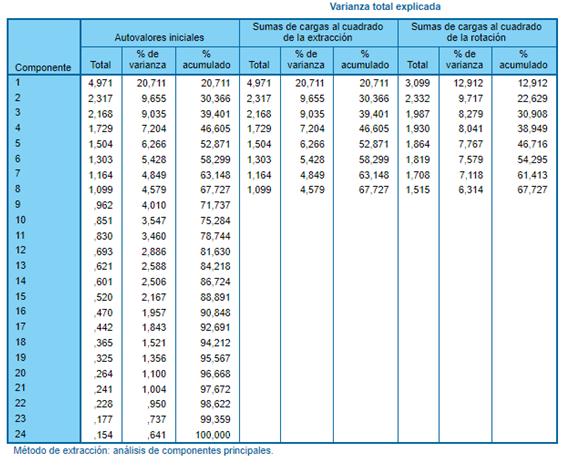
\includegraphics[width=\textwidth]{Tabla03.png}
\label{Tabla03}
\source{Autoría propia.}
\end{minipage}
\end{figure} 

- \textbf{Estudio de las puntuaciones factoriales} (solo los elementos que poseen más de tres ítems):
Factor I: A.-IoT (A3, A5), B.-Neurodiversidad (B7, B10, B11, B12), C.-Inclusión social (C13, C16, C18) y, D.-Inclusión educativa (D19, D20, D21, D22, D24). Se calcula el Alfa de Cronbach de la escala total: valor de 0.808 (24 elementos), valoración “muy bueno”. Tomamos el primer factor, el cual dispone de una fiabilidad mayor que la escala original (0.801), obteniendo así una escala final con 14 elementos, disminuyendo 10 elementos y corroborando la validez de constructo.

- \textbf{Análisis de correlación}: con el fin de proceder a la prueba que permitirá conocer la correlación entre ítems, se somete la escala Likert a la prueba de U de Mann-Whitney para dos muestras independientes, que resulta rechazar la hipótesis nula, por lo que los datos no siguen una distribución normal. Estos resultados son utilizados para realizar el análisis de correlación de Rho de Spearman \cite{fisher_metodos_1949}. A continuación, se procede a enseñar las correlaciones de ítems que tienen un alto valor significativo (0.01):

\textbf{Dimensión A (IoT):} A1>A2 (0.209), A1>A3(0.481), A1>A5 (0.157), A1>A6 (0.121), A2>A3 (0.454), A2>A4 (0.166), A2>A5 (0.343), A2>A6 (0.102), A3>A4 (0.245), A3>A5(0.341), A4>A6 (0.271), A4>A5 (0.326), A4>A6 (0.122) y A5>A6 (0.577).

Las correlaciones más altas se dan entre: A5>A6 (0.577), A5.- La IoT favorece la inclusión educativa, A6.- La IoT favorece la inclusión social y A1>A3 (0.481), A1.- La IoT permite conectar digitalmente los objetos cotidianos a internet, A3.- La IoT hace más fácil la rutina diaria.

\textbf{Dimensión B (Neurodiversidad):} B7>B8 (0.179), B7>B10 (0.301) B7>B11 (0.257), B7>B12 (0.197), B8>B9 (0.229), B8>B10 (0.128), B8>B11 (0.313), B8>B12 (0.264), B9>B10 (0.173), B9>B11 (0.111), B10>B11 (0.126), B10>B12 (0.140) y B11>B12 (0.708).

Las correlaciones más altas se dan entre: B11>B12 (0.708), B11.- La neurodiversidad favorece la inclusión educativa, B12.- La neurodiversidad favorece la inclusión social y B8>B11 (0.313), B8.- El concepto neurodiversidad hace alusión a las personas con discapacidad, B11.- La neurodiversidad favorece la inclusión educativa.

\textbf{Dimensión C (Inclusión social):} C13>C14 (0.512), C13>C15 (0.383), C13>C16 (0.420), C13>C18 (0.148), C14>C15 (0.203), C14>C16 (0.276), C15>C16 (0.178), C16>C18 (0.380) y C17>C18 (0.314).

Las correlaciones más altas se dan entre: C13>C14 (0.512), C13.-La inclusión social es la participación del segmento de la población en la vida en comunidad, C14.- La inclusión social aporta beneficios a la comunidad y C13>C16 (0.420), C13.- La inclusión social es la participación del segmento de la población en la vida en comunidad, C16.- La inclusión social permite a la persona participar plenamente en la sociedad, independientemente de su condición.

\textbf{Dimensión D (Inclusión educativa):} D19>D20 (0.417), D219>D21 (0.461), D19>D22 (0.469), D19>D23 (0.215), D19>D24 (0.358), D20>D21 (0.546), D20>D22 (0.376), D20>D23 (0.278), D20>D24 (0.301), D21>D22 (0.442), D21>D23 (0.114), D21>D24 (0.308), D22>D23 (0.327), D22>D24 (0.405), D23>D24 (0.235).

Las correlaciones más altas se dan entre: D20>D21 (0.546), D20.- La inclusión educativa favorece el rendimiento académico del alumnado, D21.- La inclusión educativa favorece las relaciones sociales entre el alumnado y D19>D22 (0.469), D19.- La inclusión educativa atiende a las necesidades educativas de los escolares, D22.- La inclusión educativa implica cambios en la educación con una visión común para todos los estudiantes.

La correlación de Rho de Spearman permite medir el grado de relación de las variables de este estudio, y demuestra la relación y traducción de cada resultado obtenido. Con todo esto, se destaca la correlación que más puntuación tiene entre B11<>B12 (0.708), B11.- La neurodiversidad favorece la inclusión educativa, B12.- La neurodiversidad favorece la inclusión social.

Se detecta esta fuerte correlación entre los ítems y se confirma la idea que exponen \textcite{messiou_inclusive_2021}, quienes afirman que las prácticas inclusivas y sociales, para que sean buenas, deben tener en cuenta la neurodiversidad.

\section{Discusión}

En la presente investigación se ha llevado a cabo una muestra de 726 sujetos (342 alumnos universitarios de ingeniería y 384 alumnos del primer curso del grado de Educación Primaria de la Universidad Autónoma de Madrid). De este modo, se ha empleado una escala Likert con 24 elementos, por consiguiente, se ha construido una tabla de operacionalización con cuatro componentes (IoT, neurodiversidad, inclusión social e inclusión educativa). La validación de contenido fue positiva y la validez de constructo se llevó a cabo mediante un análisis factorial exploratorio: KMO (0.659), Bartlett (.000), determinante ($9.650\cdot E^{-5}$), obteniendo una escala buena (0.808) y reducida (14 elementos). En este análisis, se puede destacar que los individuos encuestados consideran fundamental la inclusión social, ya que aporta beneficios a la comunidad y la inclusión educativa favorece las relaciones sociales entre el alumnado. Y no tanto que la inclusión social permite a la persona participar plenamente en sociedad, independientemente de su condición.

Por otra parte, el análisis de correlación, refleja que la correlación más alta se da entre B11>B12 (0.708), B11.- La neurodiversidad favorece la inclusión educativa, B12.- La neurodiversidad favorece la inclusión social. Y se confirma que las prácticas inclusivas y sociales, para que sean buenas, deben tener en cuenta la neurodiversidad.

Para contrastar si las poblaciones muestreadas (alumnado de ingeniería y alumnado de primer grado de Educación Primaria) son equivalentes en cuanto a las distribuciones que siguen, se emplea la prueba U de Mann-Whitney. De los 24 contrastes de hipótesis, se observan que se rechazan 19 y se aceptan 5:

\begin{enumerate}
    \item La distribución de C15.- La inclusión social es sinónimo de integración social. Es la misma entre categorías de ingeniero/a y estudiante.
    \item La distribución de D19.- La inclusión educativa atiende a las necesidades educativas de los escolares. Es la misma entre categorías de ingeniero/a y estudiante.
    \item La distribución de D20.- La inclusión educativa favorece el rendimiento académico del alumnado es la misma entre categorías de ingeniero/a y estudiante.
    \item La distribución de D21.- La inclusión educativa favorece las relaciones sociales entre el alumnado. Es la misma entre categorías de ingeniero/a y estudiante.
    \item La distribución de D22.- La inclusión educativa implica cambios en la educación con una visión común para todos los estudiantes. Es la misma entre categorías de ingeniero/a y estudiante.
\end{enumerate}

En las valoraciones de la escala Likert, existen tres dimensiones en las que los valores centrales (media y mediana) se aproximan con un error inferior al 0,1 lo cual indica que ambos valores son bastante representativos y similares a la hora de informar sobre las distribuciones:
B8.- El concepto neurodiversidad hace alusión a las personas con discapacidad.
C13.-La inclusión social es la participación del segmento de la población en la vida en comunidad.
D22.- La inclusión educativa implica cambios en la educación con una visión común para todos los estudiantes.

\section{Conclusiones}

Mediante el presente estudio se ha pretendido establecer y analizar la relación entre las siguientes cuatro dimensiones: IoT, neurodiversidad, inclusión social e inclusión educativa. Para conocer la relación entre estas variables, se ha procedido a realizar un cuestionario con escala tipo Likert, hacia una muestra de 726 sujetos (342 estudiantes del grado en Ingeniería Informática y 384 estudiantes del grado en Educación Primaria de la Universidad Autónoma de Madrid). Tras la recogida de los datos y análisis de la información, mediante el uso de un análisis factorial exploratorio, los resultados indican que nos encontramos ante una escala fiable buena de 0.808 puntos. Los sujetos investigados consideran muy importante la inclusión social por los beneficios que dicha inclusión supone para la sociedad, así como también consideran que la inclusión educativa repercute de forma óptima en las relaciones sociales que se dan entre el alumnado. De igual modo, el hecho de que exista una inclusión social potente no supone la participación absoluta de todos los miembros en la sociedad. Por su lado, el análisis de correlación realizado permite llegar a la conclusión de que es la variable neurodiversidad la que favorece la inclusión educativa, así como también la inclusión social, por lo que, la neurodiversidad es considerada elemento clave para la puesta en marcha de prácticas inclusivas. En cuanto a la dimensión IoT, los sujetos experimentales consideran que la IoT favorece la inclusión educativa determinante para una inclusión social de calidad.

Los resultados de nuestro estudio demuestran que la inclusión social es sinónimo de integración social, así como también que la inclusión educativa atiende a las necesidades de los escolares, favorece el rendimiento académico del alumnado, las relaciones sociales entre los mismos e implica cambios en la educación. Esto lleva a comprender que el futuro de la sociedad se encuentra en las aulas y en cómo en estas se lleven a cabo las prácticas inclusivas. Siendo plenamente conscientes de que todos somos en nuestra individualidad como personas, neurodiversos, (y no solo las personas con discapacidad a pesar de la creencia errónea que existe), es interesante apreciar que esta dimensión es favorecedora de una inclusión social y educativa, fundamental para construir una sociedad verdaderamente inclusiva y que la presencia de la IoT, potencia esta inclusión. Por tanto, el desarrollo y la evolución de la sociedad se encuentra, de nuevo, en manos de la educación.



\printbibliography\label{sec-bib}
% if the text is not in Portuguese, it might be necessary to use the code below instead to print the correct ABNT abbreviations [s.n.], [s.l.]
%\begin{portuguese}
%\printbibliography[title={Bibliography}]
%\end{portuguese}


%full list: conceptualization,datacuration,formalanalysis,funding,investigation,methodology,projadm,resources,software,supervision,validation,visualization,writing,review
\begin{contributors}[sec-contributors]
\authorcontribution{Sara María Extremera Sánchez}[conceptualization,validation,writing,review]
\authorcontribution{Cristina Marín Perabá}[conceptualization,investigation,writing,review]
\authorcontribution{Rocío Sanz Peinado}[conceptualization,methodology,writing,review]
\end{contributors}


\end{document}